\begin{frame}{Interprétons un dialogue}
  \begin{columns}
    \column{0.5\textwidth}
      \small
      Avec un.e partenaire, choisissez un endroit (par ex., un restaurant, un parc, le centre-ville, etc), et imaginez que vous deux, vous êtes des amis qui ne sont pas d'accord en termes des qualités de cet endroit et des choses dans cet endroit.
      Écrivez un dialogue où vous décrivez des choses avec des adjectifs opposés.
      Vous allez interpréter votre dialogue à la classe.
      \begin{itemize}
        \item[] \textbf{Modèle:}
        \item[E1:] Les trottoirs sont trop \emph{étroits} au centre-ville.
        \item[E2:] Ce n'est pas vrai! Il y a de \emph{larges} trottoirs au centre-ville.
      \end{itemize}
    \column{0.5\textwidth}
      \begin{center}
        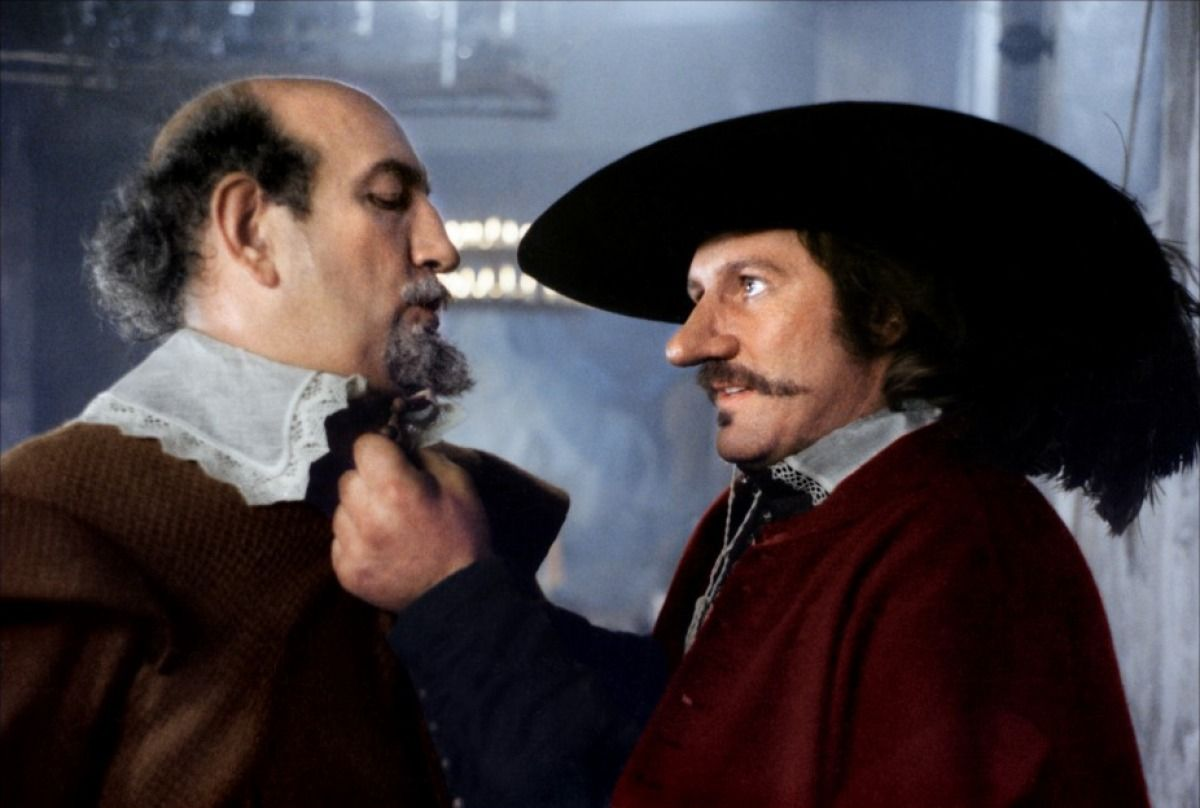
\includegraphics[scale=0.125]{cyrano.jpg} \\
        \scriptsize Gérard Depardieu dans Cyrano de Bergerac par Edmond Rostand
      \end{center}
  \end{columns}
\end{frame}